\chapter{Mix-ins}%
\label{ch:mix-ins}
\begin{quoting}
  In this chapter, you will learn about the fascinating world of sourdough
  mix-ins. Discover how these additions can elevate your bread, enhancing
  flavor, adding vibrant colors, and creating delightful textures that make
  each loaf a culinary masterpiece.
\end{quoting}

\begin{figure}[htb!]
  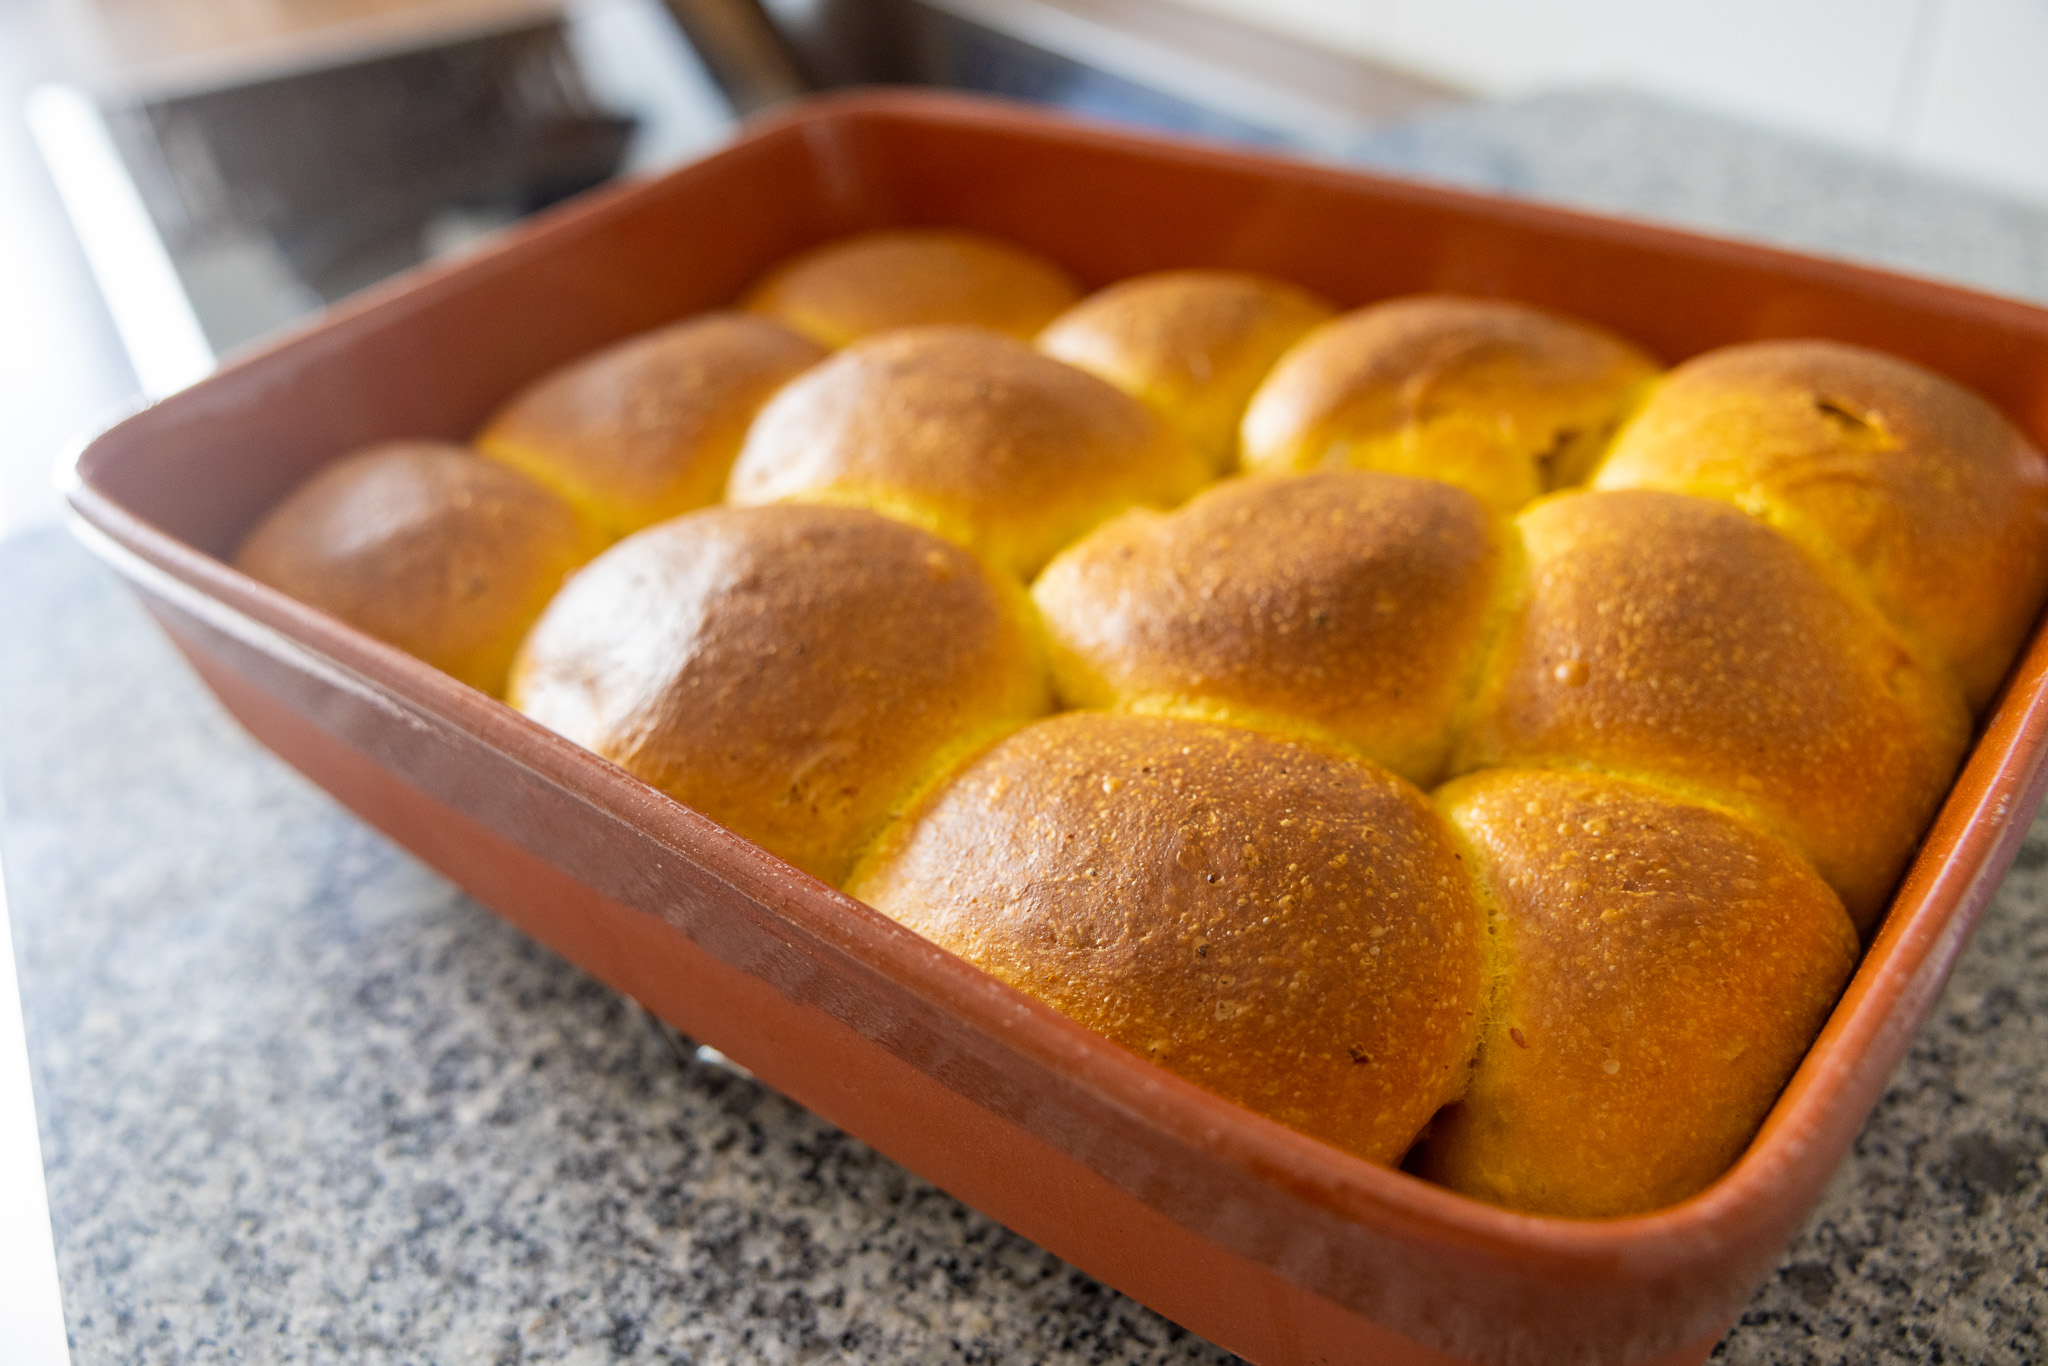
\includegraphics[width=\textwidth]{pumpkin-sourdough}
  \caption[Pumpkin sourdough softbuns]{These soft pull-apart sourdough
    buns have been made with the addition of pumpkin purée. The mashed pumpkin
    adds flavor and hydration to the dough.}%
\end{figure}

A loaf of wheat sourdough has a very pure aesthetic. Good craftsmanship and
precision transform the ingredients into simple, but delicious food. With
mix-ins, the basic recipe can become the starting point for a whole world of
modifications to try and combine. Think of the loaf of bread as a blank canvas
to express yourself.

\section{Categories}

\begin{figure}[htb!]
  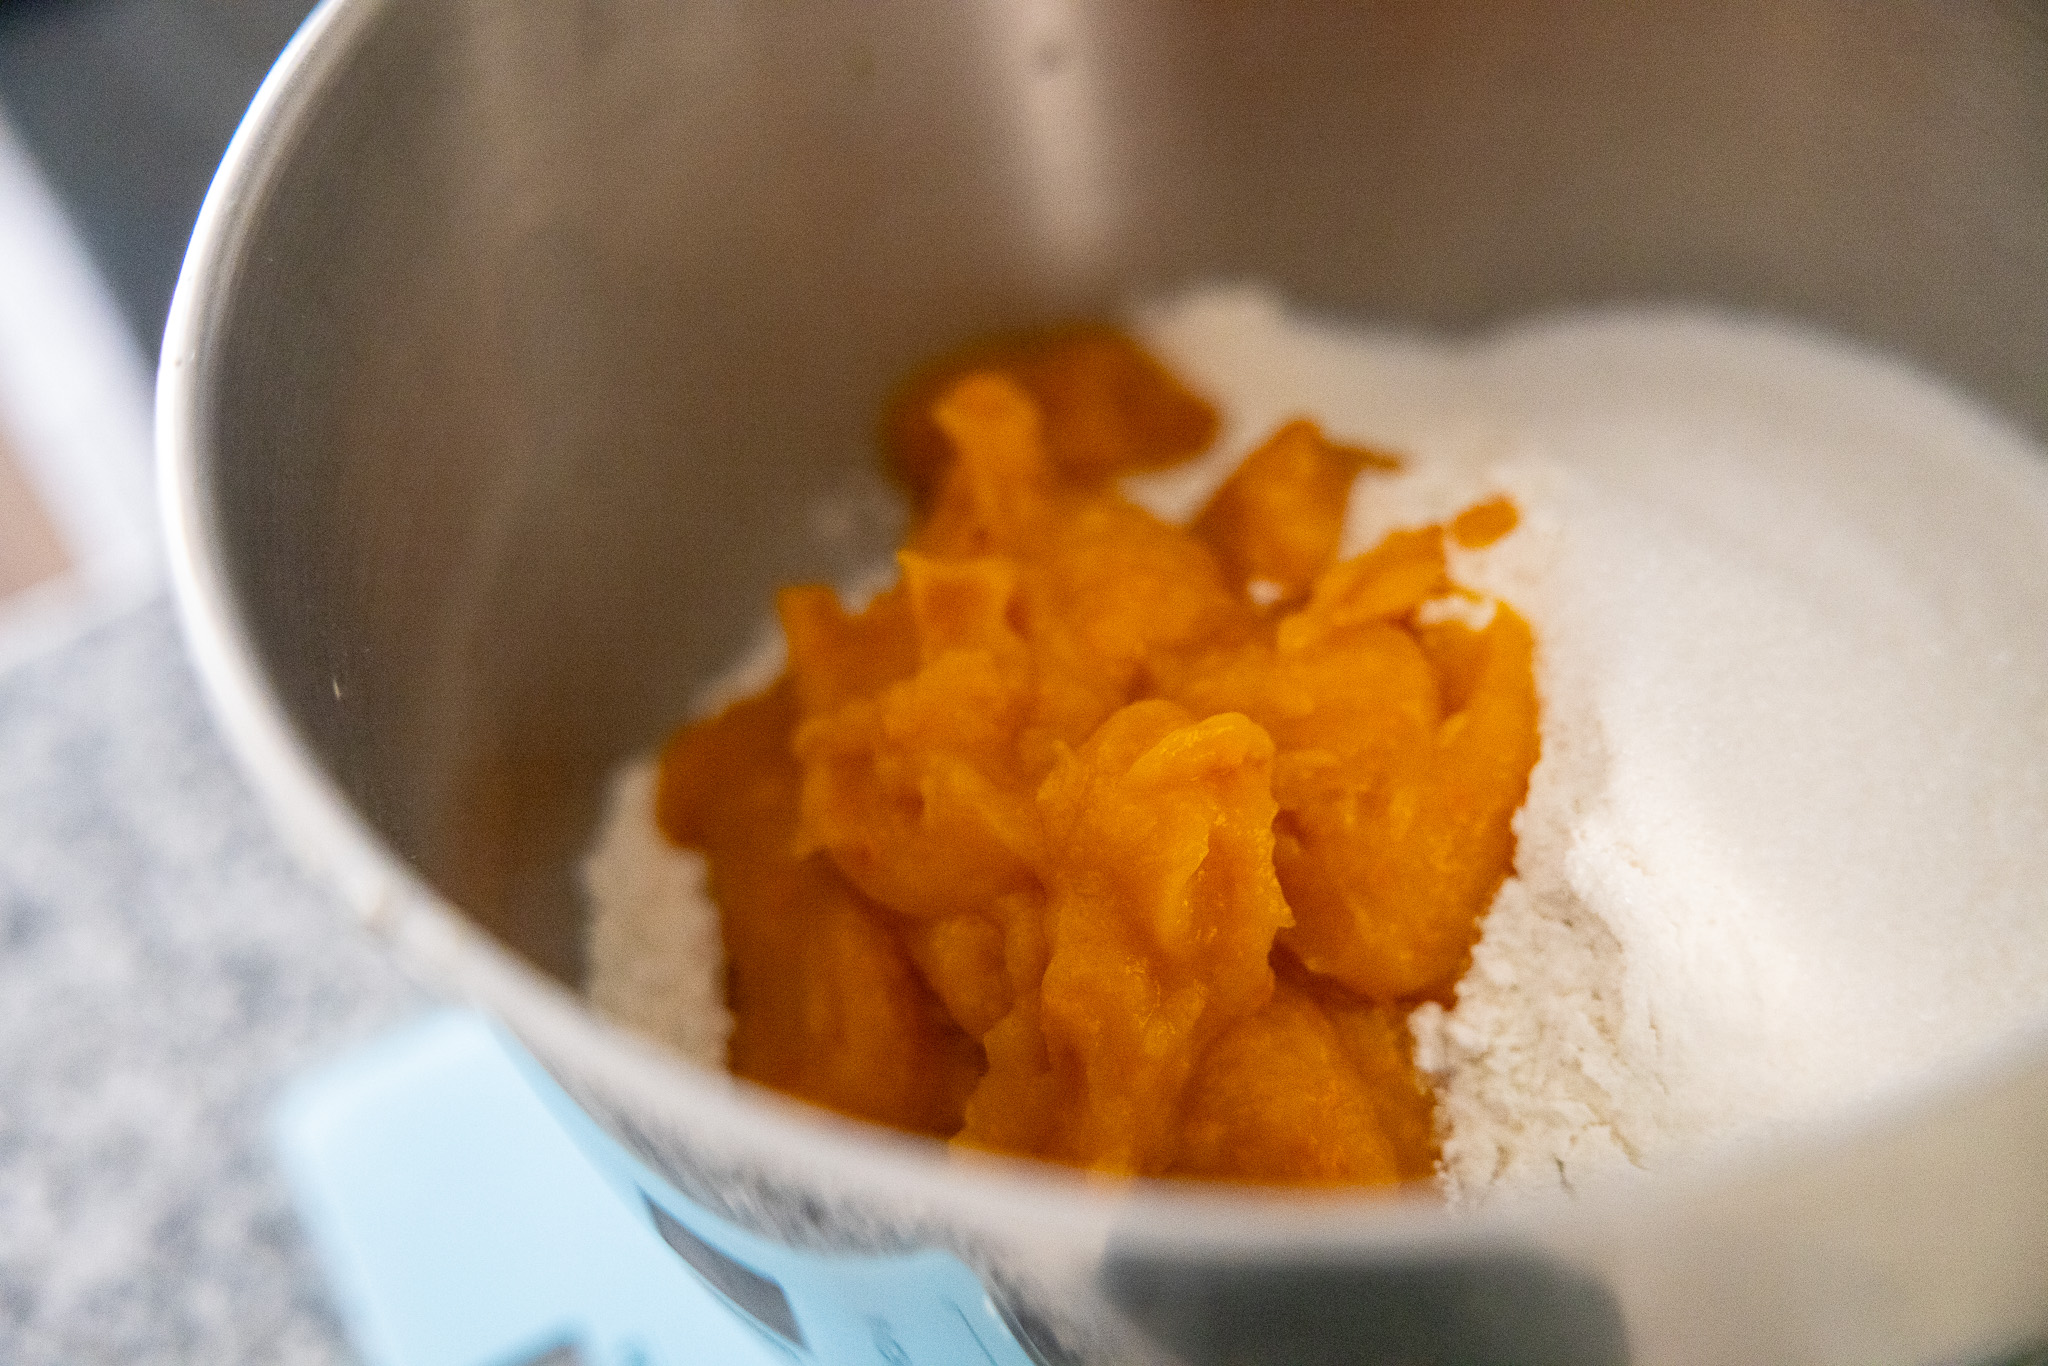
\includegraphics[width=\textwidth]{pumpkin-on-flour}
  \caption[Pumpkin puré]{A common mix-in technique is to replace some of
    the dough's water with another liquid. In this case, puréd pumpkin replaced
    some of the water. When adding puré to the dough only slowly add
    additional water as the puré slowly releases additional water to the
    dough.}%
\end{figure}

One approach to categorizing the mixins is to look at their respective shape.
However, the transition between these categories is somewhat fuzzy:

\begin{itemize}
  \item Liquids: Integrate homogeneously into the dough, may replace some of
      or all of the water. Examples: Milk, butter, oil, spinach juice, tomato
      juice, eggs
  \item Powders: Integrate homogeneously into the dough, may replace some of
      the flour. Examples: Milk powder, semolina, cocoa, spices
  \item Small bits: Individually visible in the final loaf, small enough to
      distribute somewhat evenly throughout the dough. Examples: Seeds (wheat
      berries, rye berries, poppy seeds, sesame, pumpkin seeds,
      flax seeds), whole spices (coriander)
  \item Chunks: Larger pieces that will only be present in the occasional bite
      when eating a slice of your bread. Examples: dried tomatoes, chunks of
      cheese, chunks of chocolate
\end{itemize}

Another categorization approach looks at the changes to the bread:

\begin{itemize}
  \item Flavor: Significantly changes the taste of the bread. Examples: rye
      flour, corn flour, spices, sugar.
  \item Color: Significantly changes the look of the bread. Examples: cocoa,
      squid ink, beetroot juice, tomato juice.
  \item Texture: Significantly changes the feeling in the mouth when eaten.
      Examples: Cheese (gummy), seeds (crunchy), olives (squishy chunks).
\end{itemize}

Many of the above-listed mix-ins can't be pinpointed to a single category. They
change multiple aspects of the final bread at the same time.

\begin{figure}[htb!]
  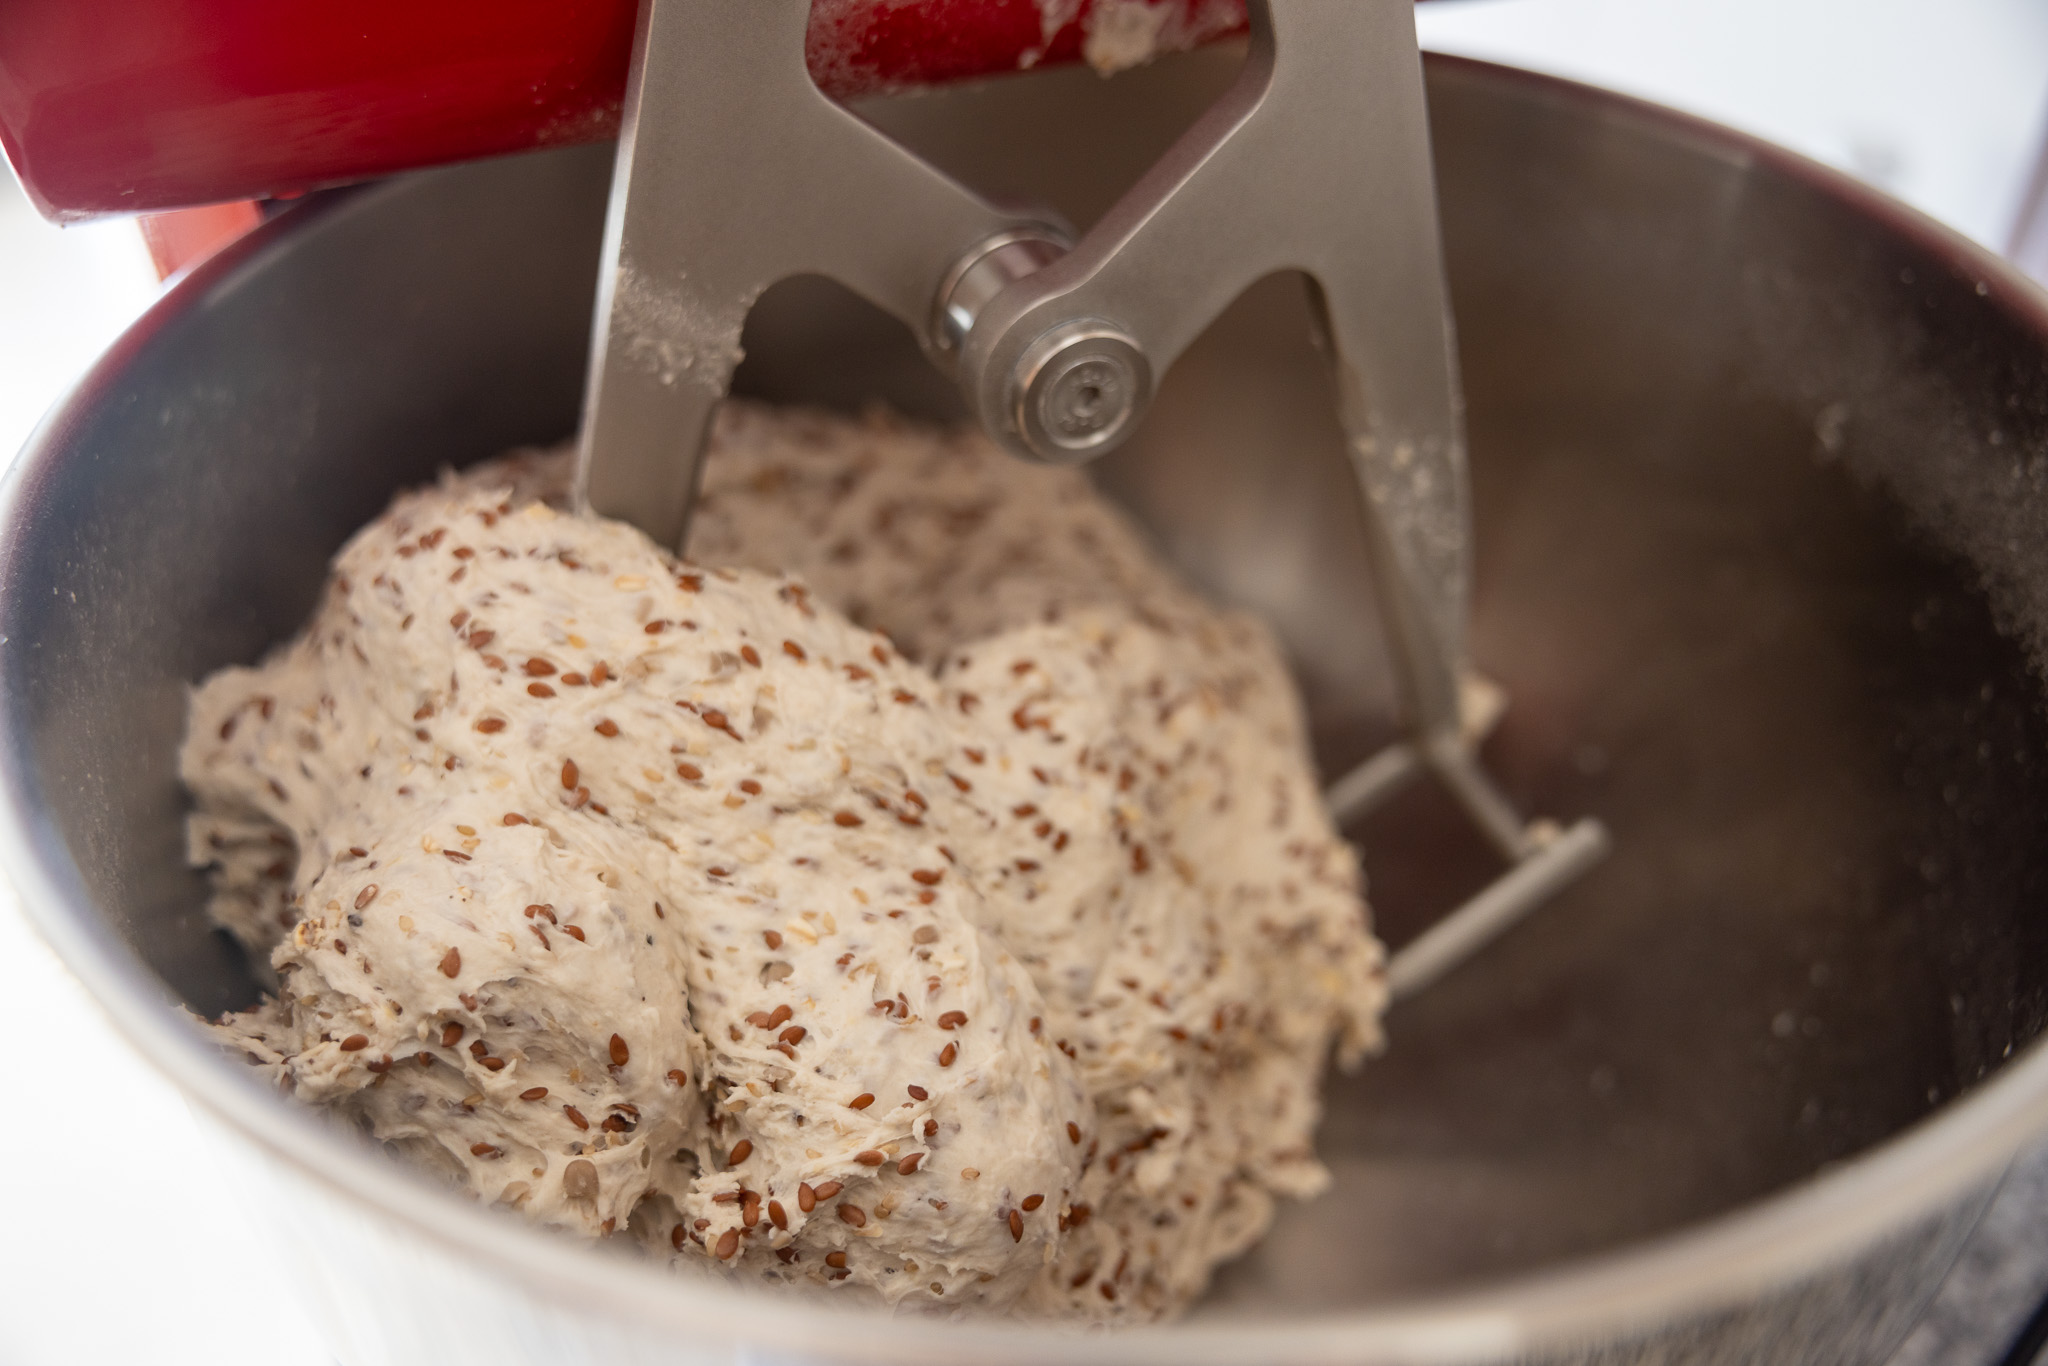
\includegraphics[width=\textwidth]{seeded-sourdough}
  \caption[Seeded sourdough]{In this case a combination of flax, sunflower and
    sesame was added to the dough. The seeds will slightly dehydrate the dough
    during fermentation and thus adding a bit more water (\qtyrange{1}{2}{\percent}) is advised.}%
\end{figure}

Mix-ins affect the structure of the dough. One aspect is the impact on
hydration. Some mix-ins absorb a lot of water when added to the dough, so you
have to increase the amount of water to achieve the same dough consistency.
The other impact is on the gluten network. Bits and chunks disrupt the gluten
network and may reduce oven spring during baking. All of this depends on the amount of mix-ins
used. A good rule of thumb is to add \qtyrange{10}{20}{\percent} of the amount
of flour in most mix-ins, reduced to around \qtyrange{1}{5}{\percent} of the
amount of flour for spices.

An important factor is also the mix-in's behavior during baking. Particularly
chunks may bake differently than dough, and either melt (cheese) leaving holes
inside, or char when peeking through the crust (\eg~vegetables). These
problems can be mitigated to some degree with the right preparation (\eg~chopping
into smaller pieces, soaking dry ingredients in water or oil first,
or squeezing out excess moisture).

\section{Examples}

The following is a list of common mix-ins and their peculiarities. They can be
combined depending on your preference.

\subsection{Flours}
These are powders. Usually, you want to just replace some fraction of the
regular bread flour. Different flours change the taste of the bread and
usually moderately affect the color.

\begin{figure}[htb!]
  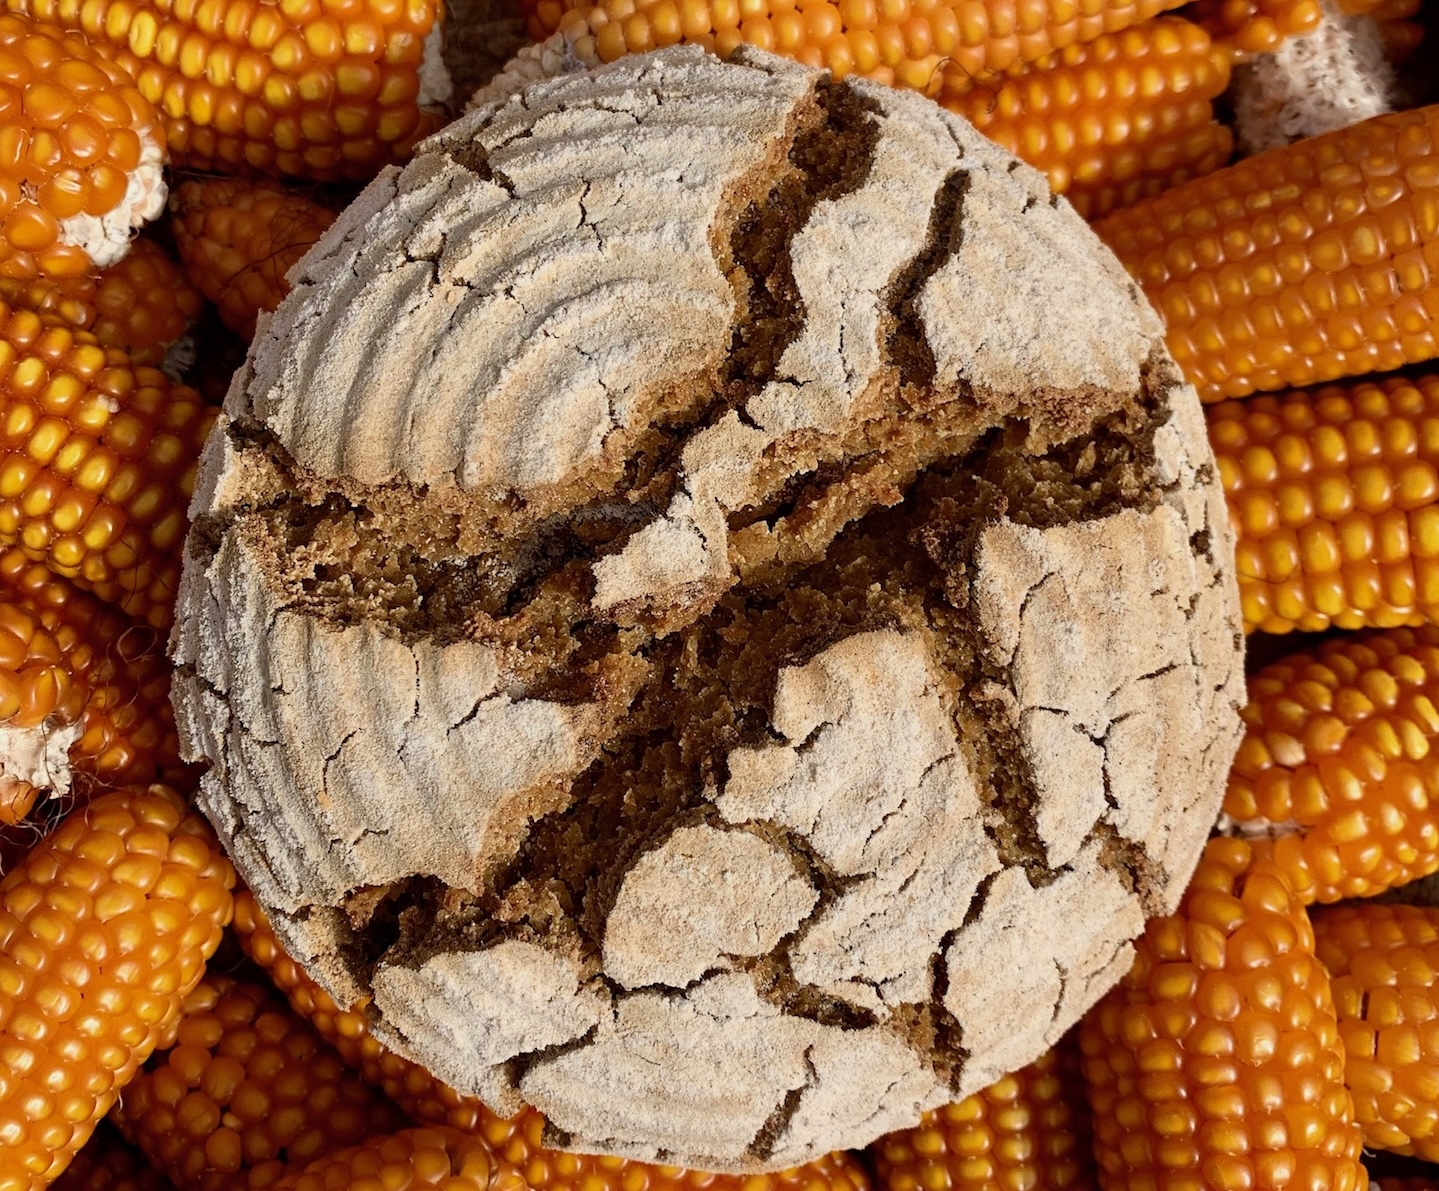
\includegraphics[width=\textwidth]{broa}
  \caption[Broa de milho]{Broa de milho is a traditional Portuguese bread
  made out of half rye and half corn flour.}%
\end{figure}

\begin{itemize}
  \item Whole wheat flour (substitute any amount, makes the bread taste more
      complex, nutty)
  \item Rye flour (very hearty, nutty, malty taste)
  \item Enzymatic malt (malty taste, improves enzymatic activity). The malt is
    a great addition when making quicker yeast-based doughs.
  \item Semolina (supports Mediterranean flavors)
  \item Cocoa (replace \qty{10}{\percent} of the flour for a black loaf, goes
      great with sweet toppings)
  \item Other non-wheat flours such as: Chickpea, corn, hemp, potato etc.
\end{itemize}

\subsection{Liquids}

Instead of using water, you can substitute it with a different liquid,
affecting taste and texture.

\begin{figure}[htb!]
  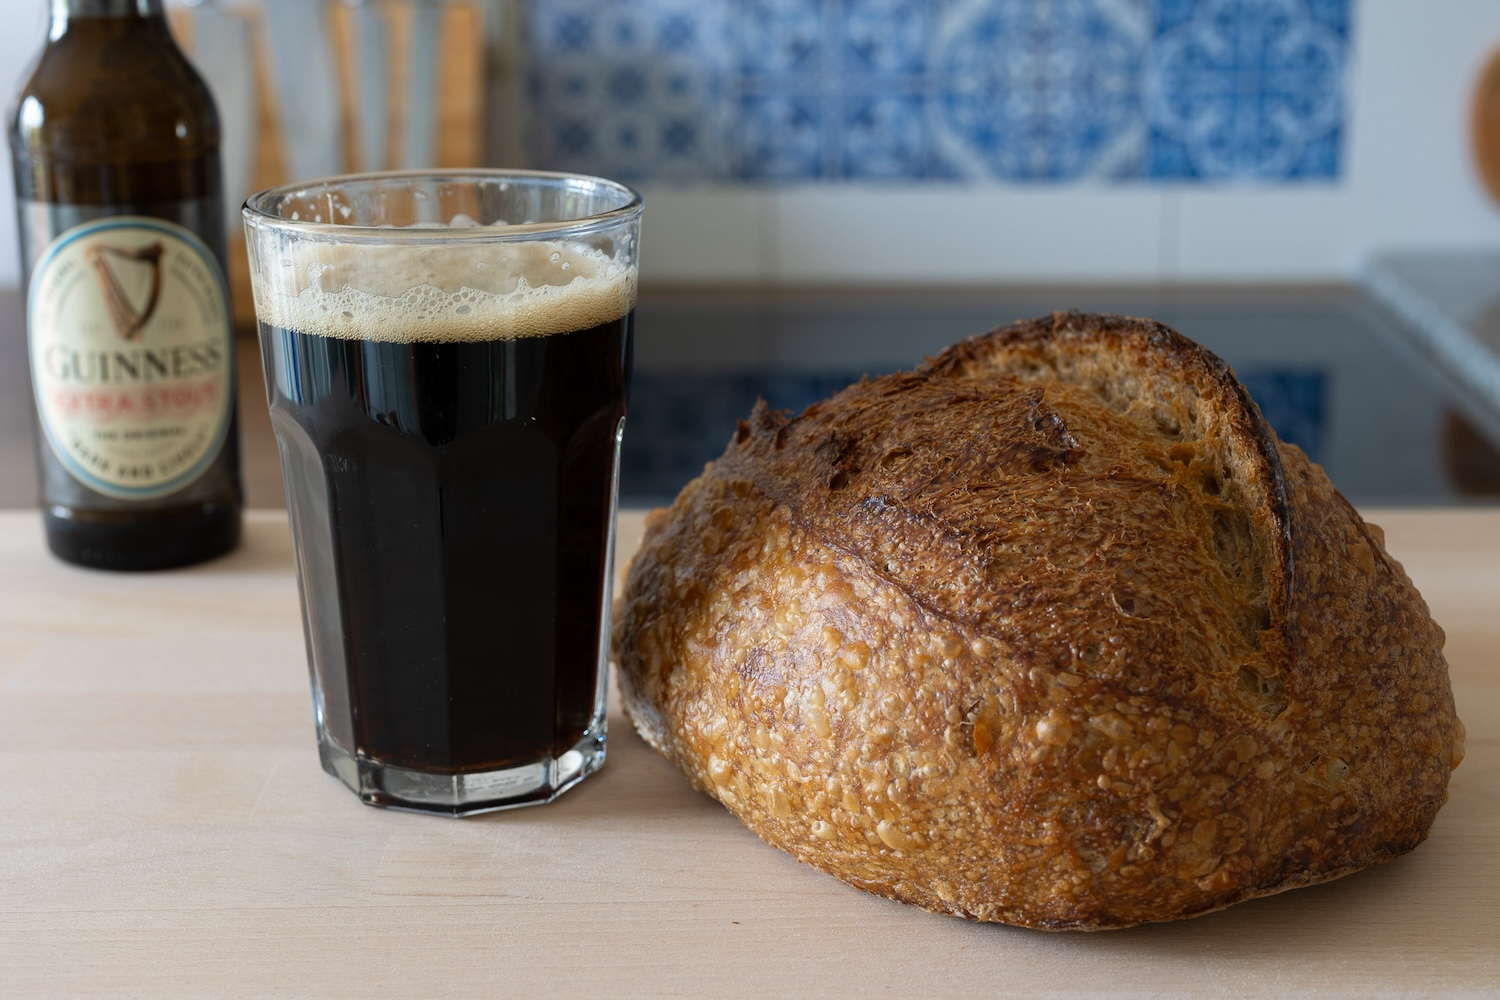
\includegraphics[width=\textwidth]{beer-bread}
  \caption[Stout beer bread]{Dark hearty stouts work excellently as a water replacement
  when making sourdough bread. The resulting loaf features a hearty malty taste}%
\end{figure}

\begin{itemize}
  \item Beer
  \item Butter
  \item Buttermilk
  \item Cereal milk (the leftover milk from eating cereals)
  \item Coffee
  \item Eggs
  \item Fruit/vegetable juices (also see Section~\ref{section:colors})
  \item Milk (for sweet, soft breads)
  \item Milk alternatives such as: Almond, oat, soy etc.
  \item Mashed potatoes
  \item Mashed sweet potatoes. Bolo do caco is a typical bread from Madeira,
    made from \qty{50}{\percent} wheat flour and \qty{50}{\percent} mashed potatoes.
  \item Olive oil (Mediterranean)
  \item Other mashed vegetables such as: Beets, pumpkin, etc.
\end{itemize}

\subsection{Colors}
\label{section:colors}
Some mix-ins will change the color and flavor of your bread. Common colorings
include:

\begin{itemize}
  \item Activated charcoal powder (black)
  \item Beetroot juice (red)
  \item Blueberry juice (blue)
  \item Blue butterfly pea flower powder (blue)
  \item Carrot juice (orange)
  \item Pear juice (pink)
  \item Spinach juice (green)
  \item Squid ink (black)
  \item Strawberry juice (red)
  \item Tomato juice (red)
\end{itemize}

\subsection{Seeds and nuts}
These are small bits, with some almost crossing into the chunk category. Some
seeds benefit from being boiled for about 10~minutes before adding them to the
dough.

\begin{figure}[htb!]
  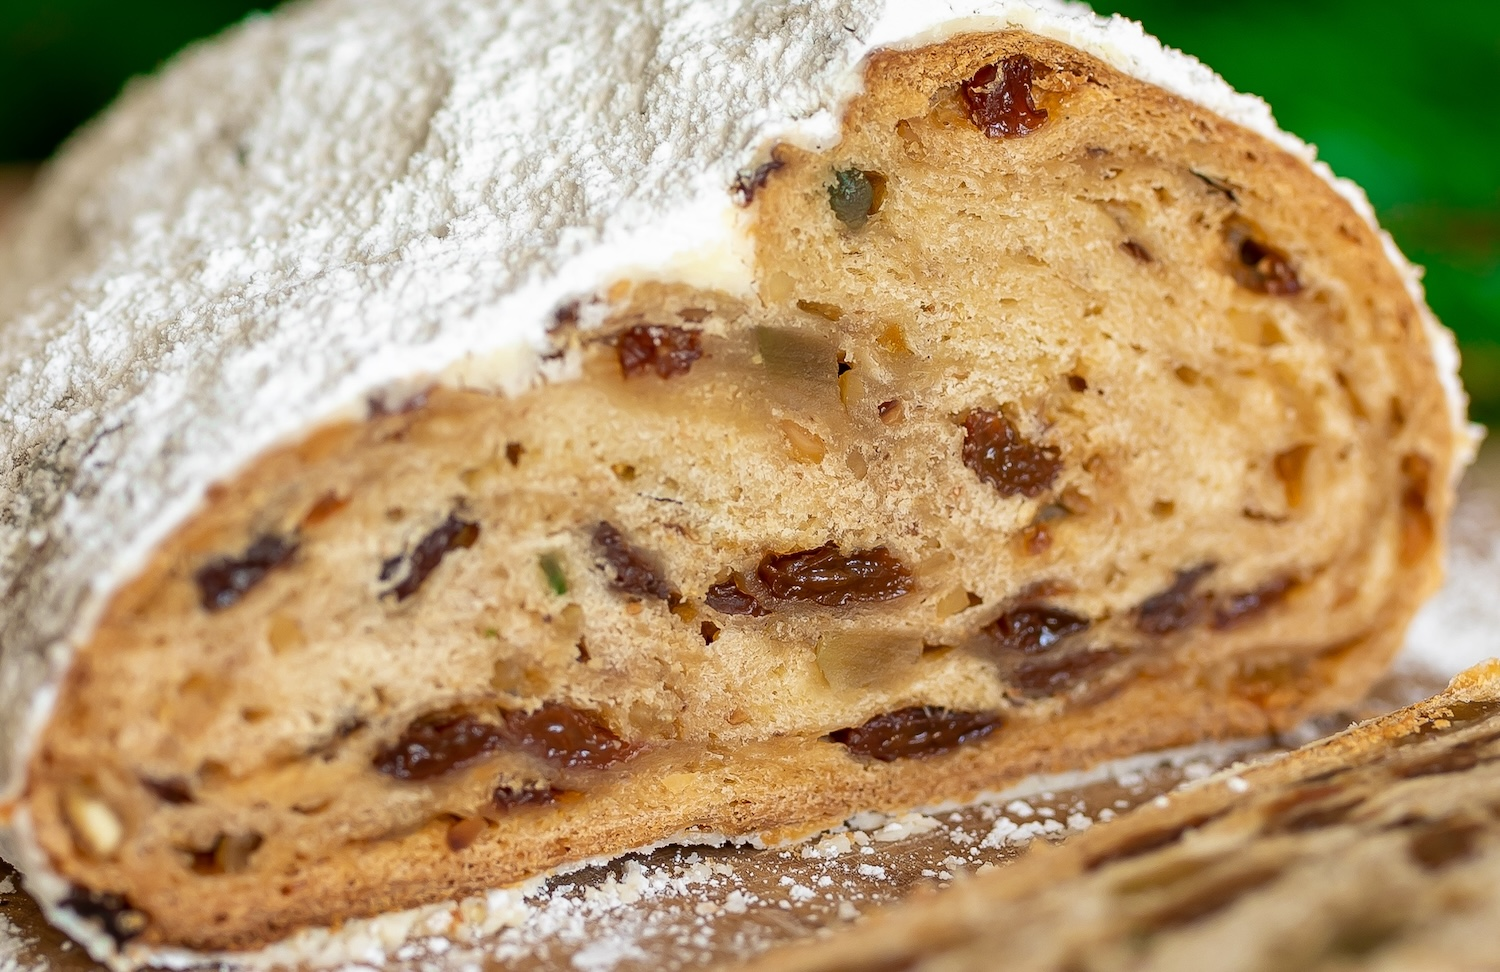
\includegraphics[width=\textwidth]{stollen-close-up}
  \caption[Stollen closeup]{The Stollen is a traditional German sweet Christmas
    bread featuring a variety of mix-ins. The dough typically contains candied lemon,
    candied orange, and raisins. The mix-ins are soaked in rum before being added to
    the dough. While the stollen matures after baking (up to \num{6} months) the candied ingredients release
    their aroma to the baked product.}%
\end{figure}

\begin{itemize}
  \item Cacao nibs
  \item Chia seed
  \item Chopped or whole nuts such as: Almonds, hazelnuts and walnuts
  \item Flaxseeds
  \item Hemp seed
  \item Poppy seed
  \item Pumpkin seed
  \item Sesame
  \item Sunflower seed
  \item Whole rye berries (boil 10 minutes)
  \item Whole wheat berries (boil 10 minutes)
\end{itemize}


\begin{figure}[htb!]
  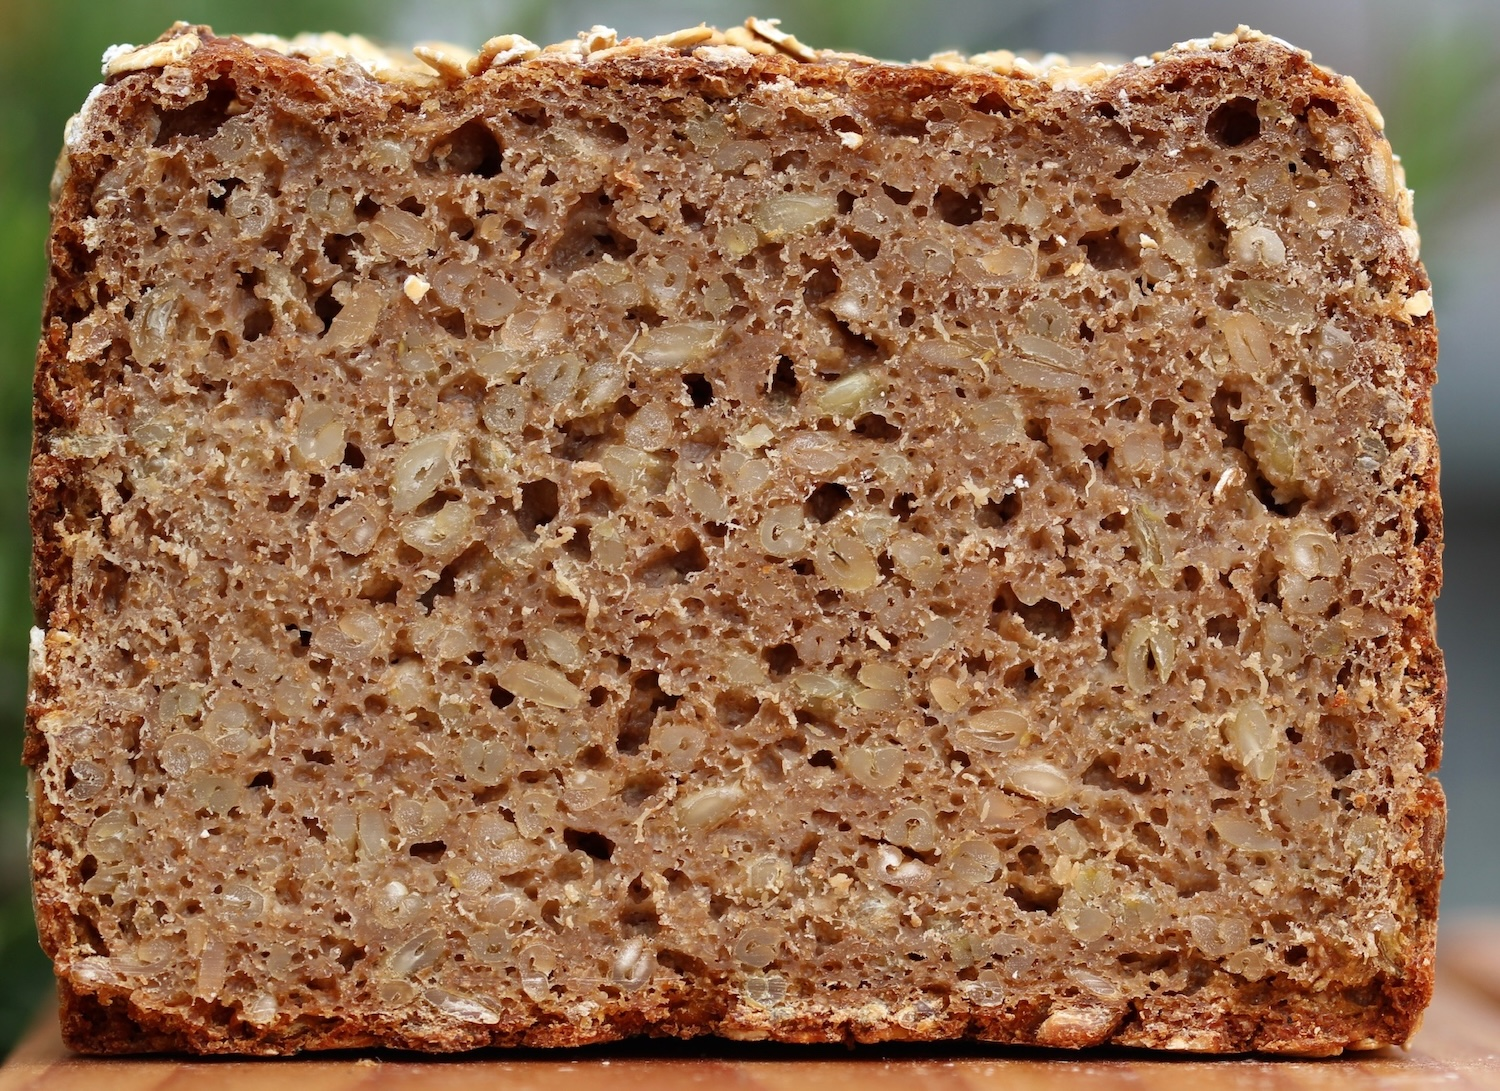
\includegraphics[width=\textwidth]{seeds-bread}
  \caption[Whole-rye with rye berries]{A sourdough bread made with half whole-rye flour and half rye berries. The
  berries are typically boiled for 10~minutes to allow them to soften a bit. When baking a loaf
  it is advised to use a thermometer to measure whether it is done baking. The final bread
  features a hearty tangy flavor and has a moist crumb.}%
\end{figure}

\subsection{Spices and flavor mix-ins}
These are mostly powders or small bits.

\begin{itemize}
  \item Blueberry skins (press through a sieve to remove juice, raw blueberries
  \item Browned onions
  \item Candied fruits such as: Lemon, orange, pineapple, etc.
  \item Cinnamon
  \item Grated hard cheese such as: Gruyère, parmesan, etc.
  \item Mediterranean herbs such as: Marjoram, oregano, rosemary, thyme, etc.
  \item Miso
  \item Molasses
  \item Sugar
  \item Spices such as: Anise, fennel, cinnamon, coriander, cumin, etc.
  \item Zests such as: Lime, Lemon, orange, etc.
\end{itemize}

\subsection{Highlights}
Mostly chunks, that add a big contrast and flavorful highlight to the basic
bread. Usually, you want to use only one (or a maximum of two) of these. The suggestions
can often be complemented by some flavor or flour mix-in.

\begin{itemize}
  \item Chocolate chunks or drops
  \item Chunks of black garlic
  \item Chunks of cheese such as: Cheddar, feta, etc.
  \item Cornflakes
  \item Dried fruits such as: Cranberries, dates, raisins, etc.
  \item Olives
  \item Pickled pepperoni
  \item Sundried tomatoes (squeeze out the oil if using pickled ones, or soak
      dried ones in water)
\end{itemize}

\subsection{Combinations}
A few combinations where multiple mix-ins complement each other:

\begin{itemize}
  \item Butter and milk. Then add cinnamon and brown sugar before shaping
  \item Cheddar and pepperoni
  \item Cheddar and jalapeño
  \item Cocoa, cacao nibs, whole hazelnuts
  \item Cranberry and walnuts
  \item Semolina, Mediterranean herbs, olives, sundried tomatoes
  \item Tomato juice instead of water with \qty{20}{\percent} rye flour
\end{itemize}

\section{Techniques}

Adding mix-ins to the dough is just the simplest approach. Add the mix-ins
directly when you knead the dough. After the first kneading wait for 30 minutes to see
if the dough has enough or too much water. In the case of whole-soaked berries
(\eg~rye or wheat) chances are that the berries will release some water and make the dough
wetter. In this case, you will want to add a bit more flour to the dough to
compensate for the high hydration.

\subsection{Adding before shaping}

\begin{figure}[htb!]
  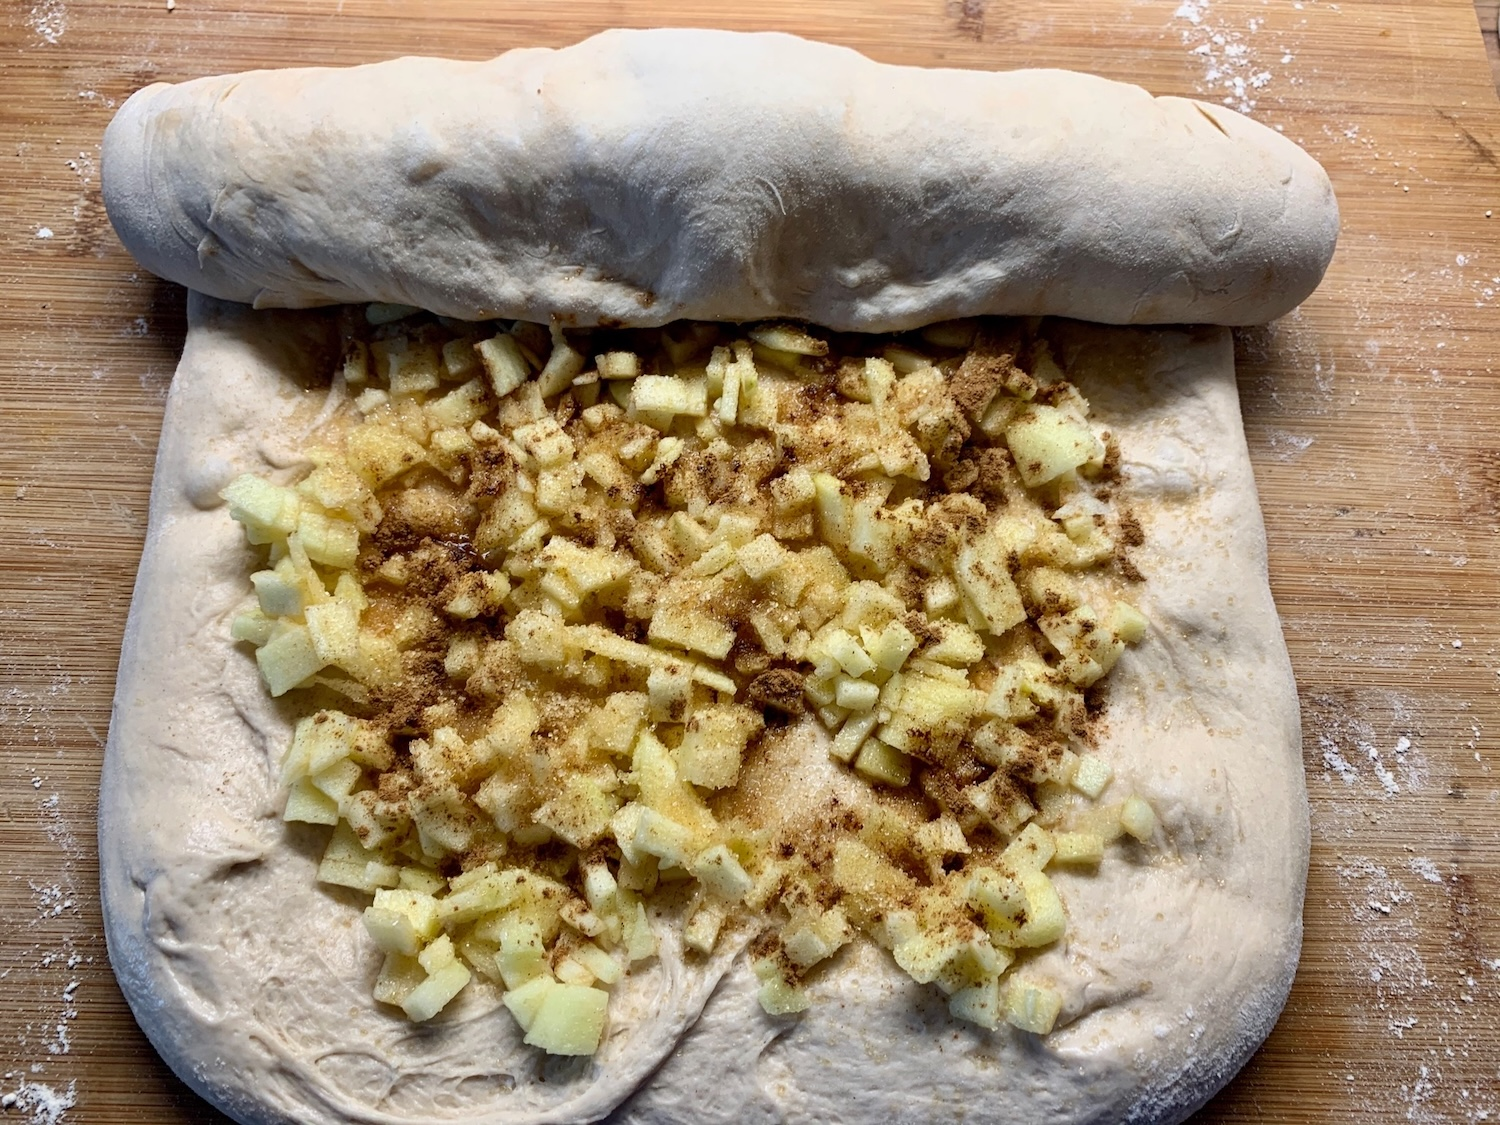
\includegraphics[width=\textwidth]{apple-swirl}
  \caption[Apple swirl buns]{A great technique is to add some of your mix-ins
  directly before shaping. In this case, a mixture of apples, cinnamon and brown
  sugar was applied. Proceed and roll the dough together. Afterward cut the roll
  into smaller pieces using a sharp knife, dough scraper or dental floss. Place
  each piece of dough next to each other in a greased bowl to allow them to be proofed.
  Proceed and bake as you would normally do. The benefit of this technique is that
  the mix-ins will not be fermented. This is typically required in the case of sugar
  since you want the final baked goods to feature sweetness. If included upon
  initial mixing most of the sugar would be fermented and the bread would not taste sweet.}%
\end{figure}

Another approach is to lay the dough out flat after the bulk fermentation.
Then using a spatula spread your ingredient over the flat dough. Continue with
your regular shaping and/or roll up the dough. When creating a roll you can
use a sharp knife to cut the dough, dental floss works great too. Afterward,
place the tiny swirls in a container to let them proof and become fluffier. This is an
excellent way to add sweet mixins as the microbes will not ferment them. When
adding sugar to the initial dough it will be fermented and the resulting dough
will not taste sweet (depending on the fermentation duration). This approach
is excellent for garlic/cheese rolls, garlic/herb rolls, and cinnamon rolls

\subsection{Covering the surface}

\begin{figure}[htb!]
  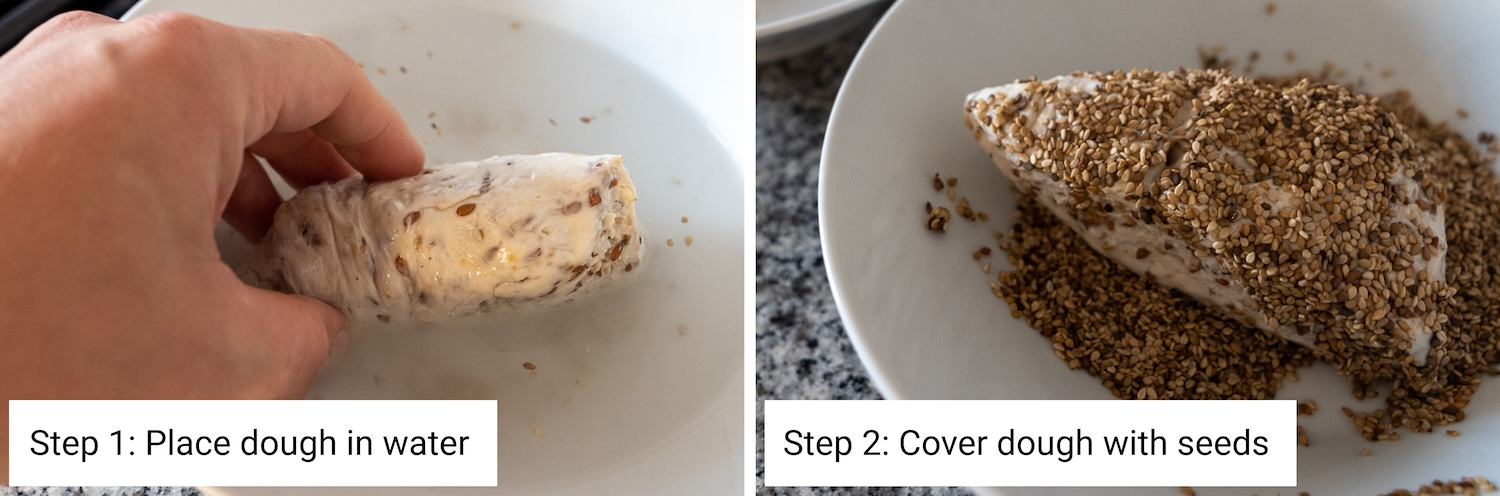
\includegraphics[width=\textwidth]{surface-seeds}
  \caption[Surface seeds]{These are chop buns which are created by chopping
    up a retarded dough into smaller pieces before baking. Then each piece of
    dough is quickly dumped in water and then rolled in a bowl of seeds.
    Afterward, the dough is directly baked in the preheated oven. These
    coverings add superb additional flavor and can be adjusted depending on
    your preference. I love adding a mixture of sunflower, flax, and
    sesame seeds.}%
\end{figure}

This works best for either powders or small bits. After shaping wrap your
coverings on the dough's surface. This works great too when covering your
banneton or loaf pan with seeds or oats. When using a loaf pan or banneton
these coverings also help to make the container stick less.

Another approach commonly used with buns is to wet the surface or dump the
dough in water. Afterward, dip the wetted piece of dough into your bowl of
mixins.  This does not work for all mix-ins, as some can't handle the high temperatures
during baking and char. Most commonly done with seeds (\eg~sesame, oats, flax-seed).

\subsection{Swirled colors}
Mix-ins that change the color of the dough bring the opportunity for even more
creativity by merging the dough before shaping.

Proceed and separate your base dough before adding a colorful ingredient. Bulk
ferment the dough in separate containers. Then Combine the two (or
more) differently colored doughs by laminating and stacking the colored sheets
of dough before the last folding, just before shaping. This way the colored
layers won't mix and the resulting dough will have differently colored and
tasting layers. \footnote{I once made an experimental dough by merging a wheat,
rye, spelt and einkorn dough into a single dough. The resulting dough was
layered featuring different colors, textures, and flavors.}
